\documentclass[11pt,a4paper]{article}
\usepackage[utf8]{inputenc}
\usepackage[T1]{fontenc}
\usepackage[english]{babel}
\usepackage{amsmath,amssymb,bm,slashed}
\usepackage{booktabs,longtable}
\usepackage{graphicx}
\usepackage[margin=2.3cm]{geometry}
\usepackage[colorlinks=true,linkcolor=blue!60!black,citecolor=blue!60!black,urlcolor=blue!60!black]{hyperref}
\usepackage{xcolor}
\newcommand{\Ap}{A'}
\newcommand{\eps}{\epsilon}
\newcommand{\KN}{\mathrm{KN}}
\newcommand{\dd}{\mathrm{d}}
\newcommand{\verdict}[1]{\textbf{\color{red!70!black}#1}}
\newcommand{\ok}[1]{\textbf{\color{green!50!black}#1}}
\title{The dark-photon production cross section at a reactor\\[2pt]
\large Lecture 1: one exact formula, three notes, eight papers, and which differences are errors}
\author{E.~L.~De Paoli\\[2pt]\small written with agent assistance (Claude Opus 5)}
\date{21 September 2026}

\begin{document}
\maketitle

\begin{abstract}
\noindent\sloppy
The documents in \texttt{apuntes/} do not compute the same thing. The Spanish note
(\texttt{Dark\_Photon\_cross\_section-1.pdf}) derives the tree-level cross section for $\gamma e^-\to \Ap e^-$ and gets
the massive case wrong: the squared amplitude, the kinematics and the kinematic range contain errors, and its final
$\dd\sigma/\dd E_{\Ap}$ is off by up to a factor 2 pointwise and crosses a propagator pole inside its own integration
range for $m_{\Ap}=1$~MeV. Each error has a one-line fix (Section~\ref{sec:note}). The \emph{v2} report
(\texttt{report\_park\_production\_v2}) has the tree-level cross section exactly right: I re-derived it with explicit Dirac
matrices and it agrees with the \emph{v2} formula, with deNiverville--Lee--Lee and with Smirnov et al.\ to
$2\times10^{-13}$. Its fold with the reactor spectrum, however, is not what Park's source equation gives: both \emph{v2}'s
Figure~2 and Park's Figure~1 have a tail equal to the photon spectrum itself, while the Compton-like convolution is
4--8 times lower above 2~MeV. The \emph{v3} report (\texttt{report\_darkphoton\_v3}) uses a different mechanism
(in-medium oscillation, Danilov et al.); it is not another way of doing the same calculation, it is the dominant production
channel, and Park's formula omits it. In TEXONO's 3--8~MeV window the two mechanisms differ by a factor $7.7$ at the same
$\eps$ (Figure~\ref{fig:two}). Park's $2/3$ detection factor is the unpolarized average and is wrong for the beam a reactor
produces; the correct factor is $\approx1$ for $m_{\Ap}\lesssim0.1$~MeV and between $0.8$ and $1$ up to 1~MeV.
\end{abstract}

\section{The question}
Three things are asked. (i)~Do the documents in \texttt{apuntes/} differ in the theoretical approach to the cross section?
(ii)~Do the \emph{final} formulas needed for the number of dark photons at a detector differ? (iii)~Are the differences
errors? The answers are: yes; yes; and mostly yes, with one exception that is not an error but an omission of physics.

Everything numerical below was produced by \texttt{work/check\_cross\_section.py} (every block ends in an
\texttt{assert}) and \texttt{work/figures\_cross\_section.py} (marimo). The run receipt is in
Section~\ref{sec:receipt}. What I derived and what I recalled is stated at each step.

\section{Setup}
Process, notation and interaction (recalled, standard):
\begin{equation}
\gamma(k)+e^-(p)\to \Ap(q)+e^-(p'),\quad m\equiv m_e,\; M\equiv m_{\Ap},\quad
\mathcal L_{\rm int}=-e\,\bar\psi\gamma^\mu\psi\,(A_\mu+\eps A'_\mu),\quad e^2=4\pi\alpha .
\end{equation}
The electron is free and at rest. Two tree diagrams ($s$- and $u$-channel electron exchange). Invariants:
\begin{equation}
s=(p+k)^2=m^2+2mE,\qquad u=(p-q)^2=m^2+M^2-2mx,\qquad t=(p-p')^2=2m(x-E),
\end{equation}
with $E$ the photon energy and $x$ the $\Ap$ energy in the lab. I use the propagator denominators
\begin{equation}
a\equiv s-m^2=2mE,\qquad b\equiv u-m^2=M^2-2mx,\qquad c\equiv m^2,\qquad d\equiv M^2 .
\label{eq:abcd}
\end{equation}

\section{Kinematics (derived, exact)}
From $(p+k-q)^2=m^2$ with $Q=|\vec q|=\sqrt{x^2-M^2}$:
\begin{equation}
M^2+2m(E-x)-2E\,(x-Q\cos\theta)=0
\quad\Longrightarrow\quad
\cos\theta=\frac{(x-m)E+mx-M^2/2}{EQ}.
\label{eq:costheta}
\end{equation}
This is transcendental in $x$ at fixed $\theta$ because $Q\neq x$. The endpoints of $x$ come from the CM two-body
momentum boosted to the lab:
\begin{equation}
x_\pm=\frac{(E+m)(s+M^2-m^2)\pm E\sqrt{\lambda(s,m^2,M^2)}}{2s},\qquad
\lambda(s,m^2,M^2)=[s-(m+M)^2][s-(m-M)^2],
\label{eq:xpm}
\end{equation}
and the threshold is $s\ge (m+M)^2$:
\begin{equation}
E_{\rm th}=M+\frac{M^2}{2m}\;:\qquad 0.1098,\;0.7446,\;1.9785~\text{MeV for }M=0.1,\,0.5,\,1~\text{MeV}.
\label{eq:thr}
\end{equation}
The threshold is \emph{not} $E=M$. At $M=1$~MeV it is twice that.

\section{The squared amplitude (derived twice)}
With $\Gamma^{\nu\mu}=\gamma^\nu(\slashed r_s+m)\gamma^\mu/a+\gamma^\mu(\slashed r_u+m)\gamma^\nu/b$,
$r_s=p+k$, $r_u=p-q$, the amplitude is $\mathcal M=\eps e^2\,\bar u(p')\Gamma^{\nu\mu}u(p)\,\varepsilon_\mu(k)\xi^*_\nu(q)$.
Averaging over the two photon polarizations and two electron spins, summing over final spins and the three $\Ap$
polarizations:
\begin{equation}
\overline{|\mathcal M|^2}=\eps^2e^4\,F,\qquad
\boxed{\;F=-2\Big(\frac ab+\frac ba\Big)+4(2c+d)\Big[\Big(\frac1a+\frac1b\Big)+c\Big(\frac1a+\frac1b\Big)^2-\frac{d}{ab}\Big]\;}
\label{eq:F}
\end{equation}
This is eq.~(36) of the \emph{v2} report. I did not take it on trust. My check builds the $4\times4$ Dirac matrices,
the explicit polarization vectors (two for the photon, $\varepsilon_{1,2}$; three for the $\Ap$, including
$\xi_L=(Q,\,x\hat q)/M$), forms $\Gamma$ numerically, and evaluates
$\tfrac14\sum\mathrm{Tr}[(\slashed p'+m)\Gamma(\slashed p+m)\bar\Gamma]$ at 60 random on-shell lab points with
$M\in[0.05,1.5]$~MeV, $E\le10$~MeV. No trace identities are used. Results:
\begin{itemize}
\item explicit polarization sum $=$ covariant $(-g_{\mu\mu'})(-g_{\nu\nu'})$ sum to $2\times10^{-13}$ (the Ward identity
$q_\nu\mathcal M^\nu=0$ holds, so the $q_\nu q_{\nu'}/M^2$ term drops);
\item numeric $=$ eq.~\eqref{eq:F} to $2\times10^{-13}$;
\item numeric $=$ deNiverville--Lee--Lee eq.~(18)--(20) to $2\times10^{-13}$;
\item $\dd\sigma/\dd x$ from eq.~\eqref{eq:F} $=$ Smirnov et al.\ eq.~(3) (with $Z=1$, $g_X=\eps e$, $x_S=1-x/E+M^2/2mE$)
to $9\times10^{-16}$.
\end{itemize}
Three independent published forms and one explicit-matrix computation agree. Eq.~\eqref{eq:F} is the tree-level
cross section. At $d=0$ it is Klein--Nishina, $F=2\,[x/E+E/x-\sin^2\theta]$ (checked with sympy).

\section{Cross sections}
Recalled: $\dd\sigma/\dd t=\overline{|\mathcal M|^2}/[16\pi(s-m^2)^2]$. Derived: $\dd t/\dd x=2m$. Hence
\begin{equation}
\boxed{\;\frac{\dd\sigma}{\dd x}=\frac{\eps^2e^4}{32\pi\,m\,E^2}\,F(a,b,c,d),\qquad a=2mE,\; b=M^2-2mx,\quad x\in[x_-,x_+]\;}
\label{eq:dsdx}
\end{equation}
Total: $\sigma=\int_{x_-}^{x_+}\dd x\,\dd\sigma/\dd x$; the \emph{v2} closed form $G(b)$ (its eq.~41) satisfies
$\dd G/\dd b=F$ (checked symbolically). Quadrature of eq.~\eqref{eq:dsdx} at $M\to0$ reproduces $\sigma_\KN$ at
$E=1,3,8$~MeV to $10^{-6}$. Mass suppression at $E=3$~MeV:
$\sigma/\sigma_\KN=0.995,\,0.886,\,0.609$ for $M=0.1,\,0.5,\,1$~MeV.

\begin{figure}[t]\centering
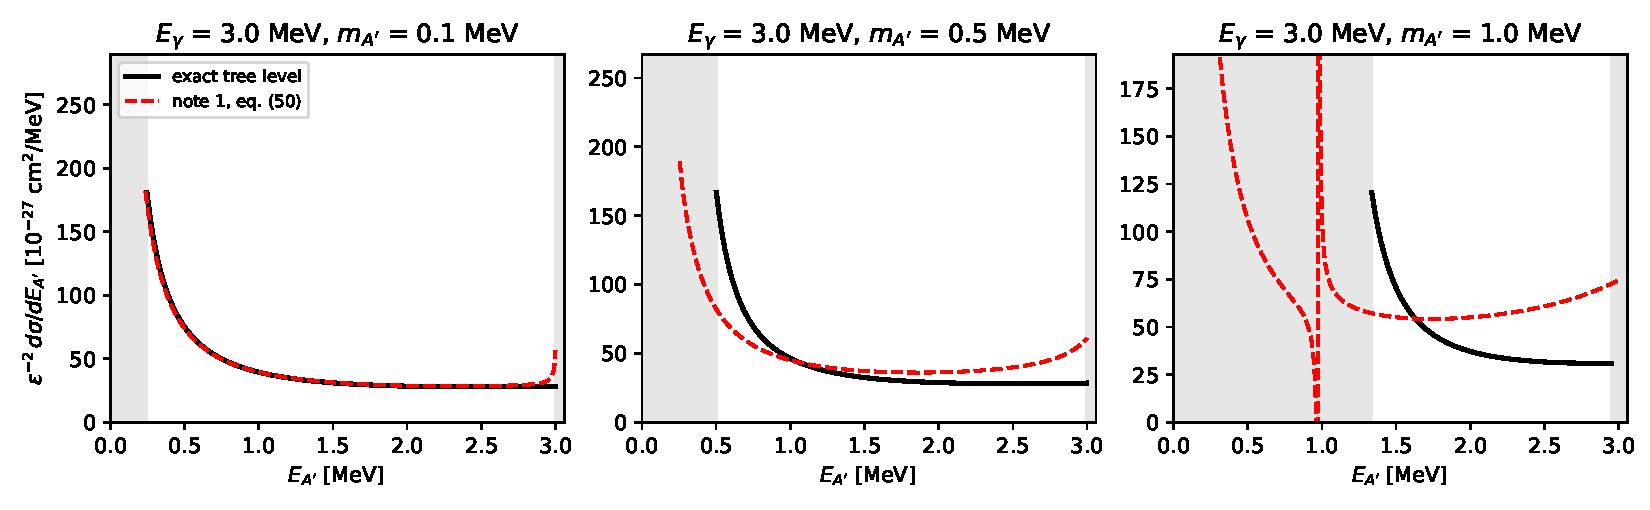
\includegraphics[width=\textwidth]{../work/fig_dsigma_dx_E3.pdf}
\caption{$\eps^{-2}\dd\sigma/\dd E_{\Ap}$ at $E_\gamma=3$~MeV. Black: eq.~\eqref{eq:dsdx}. Red dashed: the note's
eq.~(50), drawn over the range the note itself claims. Grey: outside the exact range $[x_-,x_+]$. At $M=1$~MeV the note's
formula has a pole at $E_{\Ap}=M^2/2m=0.978$~MeV ($u-m^2=0$) inside its own range.}
\label{fig:dsdx}
\end{figure}

\section{The Spanish note: what is wrong and how to fix it}
\label{sec:note}
\texttt{Dark\_Photon\_cross\_section-1.pdf} (author's name omitted) follows the right route: Feynman rules $\to$ trace $\to$ lab
phase space. Its $M=0$ total (eq.~52) is correct and equals Klein--Nishina identically (checked with sympy). Everything
that depends on $M\neq0$ needs the fixes below. The errors compound: wrong $|\mathcal M|^2$ $\times$ wrong Jacobian $\times$
wrong range.

{\small
\begin{longtable}{@{}p{2.3cm}p{4.2cm}p{3.9cm}p{4.6cm}@{}}
\toprule
Item & The note says & What is wrong & Fix \\
\midrule
\endhead
Kinematics, eqs.~(17)--(19) & solves $M^2+2m(\omega-\omega')-2\omega\omega'(1-\cos\theta)=0$, i.e.\ $|\vec k'|\approx\omega'$;
$\omega'=\frac{\omega+M^2/2m}{1+\frac{\omega}{m}(1-\cos\theta)}$ &
The algebra is right (eq.~19 does solve eq.~18) but eq.~18 itself is an approximation. At $E=3$, $x=2$, $M=1$~MeV it gives
$\cos\theta=0.832$; exact is $0.960$. &
Keep $|\vec k'|=\sqrt{\omega'^2-M^2}$: replace eq.~(18) by eq.~\eqref{eq:costheta}. Work in $\omega'$, not $\theta$; the
relation is transcendental in $\omega'$ and does not need to be inverted.\\
Threshold, Table~1 & $\omega\to M$ & Wrong: the final state must carry the photon's momentum, which costs $M^2/2m$.
Table~1 is not used in the derivation of eq.~(50), so by itself this entry is harmless; the same error enters through
the range, next row. & $E_{\rm th}=M+M^2/2m$, eq.~\eqref{eq:thr}: $1.98$~MeV for $M=1$~MeV, not $1$~MeV.\\
Range, eqs.~(24)--(25) & $\omega'\in\big[\frac{m\omega+M^2/2}{2\omega+m},\,\omega\big]$ &
Wrong at both ends: $\omega'=\omega$ is impossible for $M\neq0$, and the lower end is below the true one.
$E=3$, $M=1$: exact $[1.336,2.955]$, note $[0.312,3.000]$. This range is non-empty for every $\omega\ge M/2$, and with
$\omega'\ge M$ it gives $\omega\ge M$: it is the naive threshold of Table~1 in disguise, and this copy \emph{is} used
when eq.~(50) is integrated. &
Use $x_\pm$ of eq.~\eqref{eq:xpm} (boost of the CM momentum). For $M\to0$ it reduces to the note's limits.\\
$\overline{|\mathcal M|^2}$, eqs.~(35)--(40) & $2\eps^2e^4\big[-\frac us-\frac su+2M^2(\frac1s+\frac1u)-\frac{M^4}{4}(\frac1s+\frac1u)^2su\big]$
($s,u$ = propagator denominators) &
Off by $-39\%$ to $+33\%$ against eq.~\eqref{eq:F}. Eqs.~(35)--(36) drop the $m^2$ terms ``$O(m_e^2/s)$'', but
$m_e^2/s$ is not small at MeV energies: at $M=0$ exactly $8m^2(\frac1a+\frac1b)+8m^4(\frac1a+\frac1b)^2$ is missing, and
that is what produces the $-\sin^2\theta$ of Klein--Nishina. Eq.~(39) is not the trace it names. &
Replace eq.~(40) by eq.~\eqref{eq:F} with $a=s$, $b=u$ of the note's notation. Keep every power of $m$; there is no
regime in this problem where $m_e\ll\sqrt s$.\\
$\dd\sigma/\dd\Omega$, eqs.~(43)--(46) & KN bracket $+M^2 f(s,u)$, $f=\frac{2}{s+u}(1-\frac{m^2M^2}{su})$, massless
phase-space factor $(\omega'/\omega)^2$ &
Does not follow from eq.~(40): the $-\sin^2\theta$ term needs the $m^2$ terms dropped earlier. The phase-space factor
for a massive final particle is $|\vec k'|\omega'/\ldots$, not $\omega'^2$. &
Do not go through $\dd\Omega$. Use the invariant form $\dd\sigma/\dd t=\overline{|\mathcal M|^2}/[16\pi(s-m^2)^2]$
and $\dd t=2m\,\dd\omega'$; this gives eq.~\eqref{eq:dsdx} with no angular Jacobian at all.\\
Jacobian, eqs.~(47)--(48) & $\dd\Omega/\dd\omega'=\frac{2\pi}{\omega'^2}(m+\frac{M^2}{2\omega})$ &
Derived from the approximate eq.~(20); the exact one has $|\vec k'|$ in it. & Not needed once eq.~\eqref{eq:dsdx} is used.\\
Final $\dd\sigma/\dd\omega'$, eq.~(50) & $\frac{\pi\eps^2\alpha^2}{m\omega^2}(1+\frac{M^2}{2m\omega})[\ldots]$ &
Off by up to $2\times$ pointwise (Fig.~\ref{fig:dsdx}); has a pole at $\omega'=M^2/2m$ ($u=0$ in the note's notation)
which lies inside the note's range for $M=1$~MeV ($0.978\in[0.312,3]$), so the total does not exist there. Over the
exact range the total is $0.5\%$, $7\%$, $36\%$ too high for $M=0.1$, $0.5$, $1$~MeV. &
Eq.~\eqref{eq:dsdx} on $[x_-,x_+]$. The pole is outside the exact range for every $M<2m$.\\
\bottomrule
\end{longtable}}

\paragraph{Which of these errors matters for the number of dark photons.} Folding the note's eq.~(50), on the note's
range, with Park's spectrum through eq.~\eqref{eq:park1} ($\sigma_{\rm tot}=\sigma_\KN$, 1~GW, $\eps=1$) and comparing
with the same fold of eq.~\eqref{eq:dsdx} on $[x_-,x_+]$ (\texttt{work/check\_eq50\_fold.py}):
\begin{center}\small
\begin{tabular}{@{}lcccc@{}}
\toprule
$M$ [MeV] & photons with $M<\omega<E_{\rm th}$ & \multicolumn{2}{c}{$\dd\dot N/\dd E_{\Ap}$, note/exact} & $\dot N_{\Ap}$(3--8~MeV), note/exact\\
 & & at 3~MeV & at 5~MeV & \\
\midrule
0.1 & 1.1\% & 1.06 & 1.05 & 1.05\\
0.5 & 23.6\% & 1.48 & 1.43 & 1.46\\
1.0 & 65.9\% & 2.05 & 1.90 & 1.99\\
\bottomrule
\end{tabular}
\end{center}
In the 3--8~MeV window the threshold/range error contributes nothing: an $\Ap$ of $E_{\Ap}\ge3$~MeV comes from a photon
of $\omega\ge3$~MeV, and all of those are above threshold for $M\le1$~MeV ($\omega'_{\max}=\omega$ instead of $x_+$
moves the lower photon energy from $3$ to $3.05$~MeV). The factors $1.05$, $1.46$, $1.99$ come from eq.~(50) itself: the
$|\mathcal M|^2$ without its $m^2$ terms and the massless Jacobian. That is the error to fix for TEXONO's CsI.
The range error matters at low $E_{\Ap}$: for $M=1$~MeV, $66\%$ of the photons above $1$~MeV are below the true threshold
and the note lets them produce $\Ap$; for $E_{\Ap}$ between $0.31$ and $1.34$~MeV eq.~(50) integrates over a
kinematically forbidden region that contains the pole at $0.978$~MeV (at $E_{\Ap}=1$~MeV: exact $0$, note
$1.5\times10^{21}$~MeV$^{-1}$s$^{-1}$). That matters for a low-threshold detector such as TEXONO's PCGe, not for the CsI.

\paragraph{Minimal correction of eq.~(50).} Replace the bracket $[\ldots]$ by $F/2$ with $a=2m\omega$, $b=M^2-2m\omega'$,
$c=m^2$, $d=M^2$; replace the prefactor $\frac{\pi\eps^2\alpha^2}{m\omega^2}(1+\frac{M^2}{2m\omega})$ by
$\frac{\pi\eps^2\alpha^2}{m\omega^2}$, i.e.\ $\dd\sigma/\dd\omega'=\eps^2e^4F/(32\pi m\omega^2)$; replace the range by
$[x_-,x_+]$. The threshold then comes out by itself and the pole is outside the range for every $M<2m$.

\noindent With those replacements the note's Section~9 summary becomes: $\cos\theta$ from eq.~\eqref{eq:costheta},
$\overline{|\mathcal M|^2}=\eps^2e^4F$ with eq.~\eqref{eq:F}, $\dd\sigma/\dd\omega'$ from eq.~\eqref{eq:dsdx}, range
$[x_-,x_+]$ from eq.~\eqref{eq:xpm}, threshold eq.~\eqref{eq:thr}. Its Section~8 (the $M=0$ total) stays as it is.

\begin{figure}[t]\centering
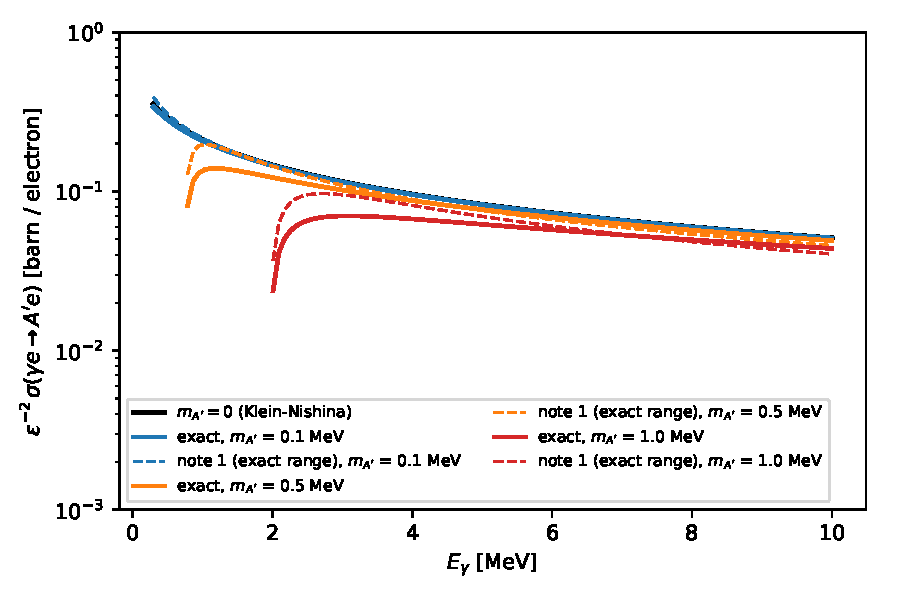
\includegraphics[width=0.62\textwidth]{../work/fig_sigma_total.pdf}
\caption{Total production cross section per electron, $\eps=1$. Solid: eq.~\eqref{eq:dsdx} integrated over
$[x_-,x_+]$; the $M=0$ curve is Klein--Nishina. Dashed: the note's integrand integrated over the \emph{exact} range
(over its own range it diverges for $M=1$~MeV).}
\end{figure}

\section{The v2 report: correct, and what it does not settle}
\texttt{report\_park\_production\_v2\_en.pdf} derives eq.~\eqref{eq:F}, eq.~\eqref{eq:dsdx}, the exact range
\eqref{eq:xpm} and the threshold \eqref{eq:thr}, with polynomial and matrix checks. All of that is confirmed here
independently. It then folds the cross section with Park's spectrum through Park's source equation
\begin{equation}
\frac{\dd\dot N_{\Ap}}{\dd x}=\int\dd E\,S_\gamma(E)\,\frac{1}{\sigma_{\rm tot}(E)}\frac{\dd\sigma(E,x)}{\dd x},\qquad
S_\gamma=0.58\times10^{18}\,\frac{P}{\rm MW}\,e^{-E/0.91\,{\rm MeV}}\ {\rm s^{-1}MeV^{-1}},
\label{eq:park1}
\end{equation}
with $\sigma_{\rm tot}=\sigma_\KN$ as Park does. I reproduce the photon integral,
$\int_{1\,\rm MeV}^\infty S_\gamma=1.7588\times10^{20}$~s$^{-1}$ at 1~GW (Park prints $1.76\times10^{20}$).

The fold itself is where \emph{v2} and Park part company with eq.~\eqref{eq:park1}. Evaluating eq.~\eqref{eq:park1}
with the triple-checked cross section, at 1~GW, $\eps=1$, $M=0.1$~MeV (script section 9):
\begin{center}\small
\begin{tabular}{@{}lcccc@{}}
\toprule
$E_{\Ap}$ [MeV] & eq.~\eqref{eq:park1} & $S_\gamma(E_{\Ap})$ & Park Fig.~1 (read by eye) & \emph{v2} Fig.~2 (read by eye)\\
\midrule
1 & 0.108 & 0.193 & $\approx0.40$ & $\approx0.10$\\
2 & 0.017 & 0.064 & $\approx0.065$ & $\approx0.065$\\
3 & 0.0036 & 0.021 & $\approx0.022$ & $\approx0.020$\\
4 & 0.0009 & 0.0072 & $\approx0.007$ & $\approx0.005$\\
\bottomrule
\end{tabular}\\[2pt]
units $10^{21}$~MeV$^{-1}$s$^{-1}$
\end{center}
Above 2~MeV Park's curve is the photon spectrum $S_\gamma$ to within the reading error, and \emph{v2}'s curve follows
Park (that is its ``4\% median residual''). Eq.~\eqref{eq:park1} cannot give that: a photon of energy $E$ spreads its
$\Ap$ over $[x_-,x_+]$ with density $\sigma_\KN^{-1}\dd\sigma/\dd x\approx0.15$--$0.4$~MeV$^{-1}$, so
$\dd\dot N/\dd x\approx0.3\int_x^\infty S_\gamma\approx0.27\,S_\gamma(x)$ at $x=2$~MeV, which is what the script finds
(bounds $[0.009,0.025]$ contain $0.017$). The integral of eq.~\eqref{eq:park1} over $x$ equals the number of photons
to $0.1\%$, so the normalisation is not the issue; the shape is. Whatever Park's generator did, it is not
eq.~\eqref{eq:park1}; and since \emph{v2} matches Park rather than eq.~\eqref{eq:park1}, its fold is not confirmed
either. Its cross section is. I did not have \emph{v2}'s code to find where its fold departs.

The $\sigma_{\rm tot}$ in eq.~\eqref{eq:park1} is a real difference between papers: Park uses the free-electron
Klein--Nishina cross section; Smirnov et al., NEON and Lou--Wu use the XCOM total (photoelectric $+$ Compton $+$
pair) for the core material. Only the total makes sense as a normalisation --- any interaction removes the photon.
For uranium the ratio $\sigma_\KN N_A Z/A\,/\,(\mu/\rho)_{\rm NIST}$ tabulated in \emph{v2} is $0.62$, $0.60$, $0.43$,
$0.29$ at $1,3,5,8$~MeV (recalled from \emph{v2}'s table, not recomputed here). Park's choice overestimates the
Compton-like yield by $1.6$--$3.5$ in the TEXONO window.

\section{The v3 report and the two mechanisms}
\label{sec:two}
\texttt{report\_darkphoton\_v3\_en.pdf} does not use a Compton cross section for production at all. It uses
Danilov--Demidov--Gorbunov:
\begin{equation}
\begin{aligned}
&\frac{\dd\dot N_X}{\dd E}=P_{\gamma\to X}(E)\,\frac{\dd\dot N_\gamma}{\dd E},\qquad
P_{\gamma\to X}=\frac{\eps^2m_X^4}{(\Delta m^2)^2+E^2\Gamma^2},\\
&\Delta m^2=\sqrt{(m_X^2-m_\gamma^2)^2+4\eps^2m_X^2(m_X^2+m_\gamma^2)},
\end{aligned}
\label{eq:danilov}
\end{equation}
with $m_\gamma^2=4\pi\alpha n_e/m_e\approx(20\,{\rm eV})^2$ and $1/\Gamma\approx10$~cm. For $m_X\gg m_\gamma$ and
$m_X^2\gg E\Gamma\sim(3\,{\rm eV})^2$ this is $P=\eps^2$ with $E_X=E_\gamma$.

This is a different mechanism, not a different derivation of the same one. In the basis where $\Ap$ couples to the
current with $\eps e$, eq.~\eqref{eq:danilov} in the $\eps^2$ limit is direct emission of an $\Ap$ at every vertex that
emits a reactor photon (nuclear de-excitation, capture, annihilation): probability $\eps^2$ per photon, same energy,
no recoil. Lou--Wu 2026 compute exactly this for the strongest capture lines and find it beats the Compton-like
channel. Park's eq.~\eqref{eq:park1} is instead a \emph{secondary} process: a photon that already exists Compton-scatters
and the outgoing photon is replaced by an $\Ap$, with the Compton energy loss. Demidov--Gorbunov--Polonski 2025 treat
this same secondary channel inside the oscillation formalism (``Compton-scattered photons'') and find an enhancement
factor $f(E)=1.2$ at 2~MeV falling towards 1 above 4~MeV.

The two mechanisms give the same order of magnitude in total ($\approx\eps^2N_\gamma$) but very different spectra.
Computed here with Park's spectrum, $P=1$~GW, $\eps=1$, counting $\Ap$ with $x\in[3,8]$~MeV:
\begin{equation}
\begin{aligned}
\dot N^{\rm (A)}_{[3,8]}&=2.53\times10^{18}\ {\rm s^{-1}}\quad(\text{Compton-like, eq.~\eqref{eq:park1}, }\sigma_{\rm tot}=\sigma_\KN),\\
\dot N^{\rm (B)}_{[3,8]}&=1.95\times10^{19}\ {\rm s^{-1}}\quad(\text{eq.~\eqref{eq:danilov}, }P=\eps^2),
\end{aligned}
\end{equation}
ratio $0.130$, essentially independent of $M$ between $0.1$ and $1$~MeV (Figure~\ref{fig:two}). Mechanism~A is
not small everywhere: below $0.5$~MeV it is comparable to B, because that is where the Compton-scattered $\Ap$ from
the many 1--2~MeV photons land. In the TEXONO window it is $13\%$ of B. That $13\%$ is the same size as Demidov et al.'s $f(E)-1$ at 3--4~MeV. It is nowhere near the factor 10 claimed by Du et al.\ 2024; Demidov et al.\
trace Du's factor to treating each scattering as a full wave-function collapse (missing the factor $1/2$ and
$\Gamma_{\rm abs}\to\Gamma_{\rm tot}$). I did not rerun either Monte Carlo; the single-scattering estimate above is
consistent with Demidov and inconsistent with Du, which is as far as this check goes.

So: Park's approach (and the \emph{v2} report, and NEON 2025 which copies Park's eq.~2) computes the subleading channel
and omits the leading one. That is the biggest difference among the final formulas in \texttt{apuntes/}, and it is an
omission of physics, not an algebra error.


\begin{figure}[t]\centering
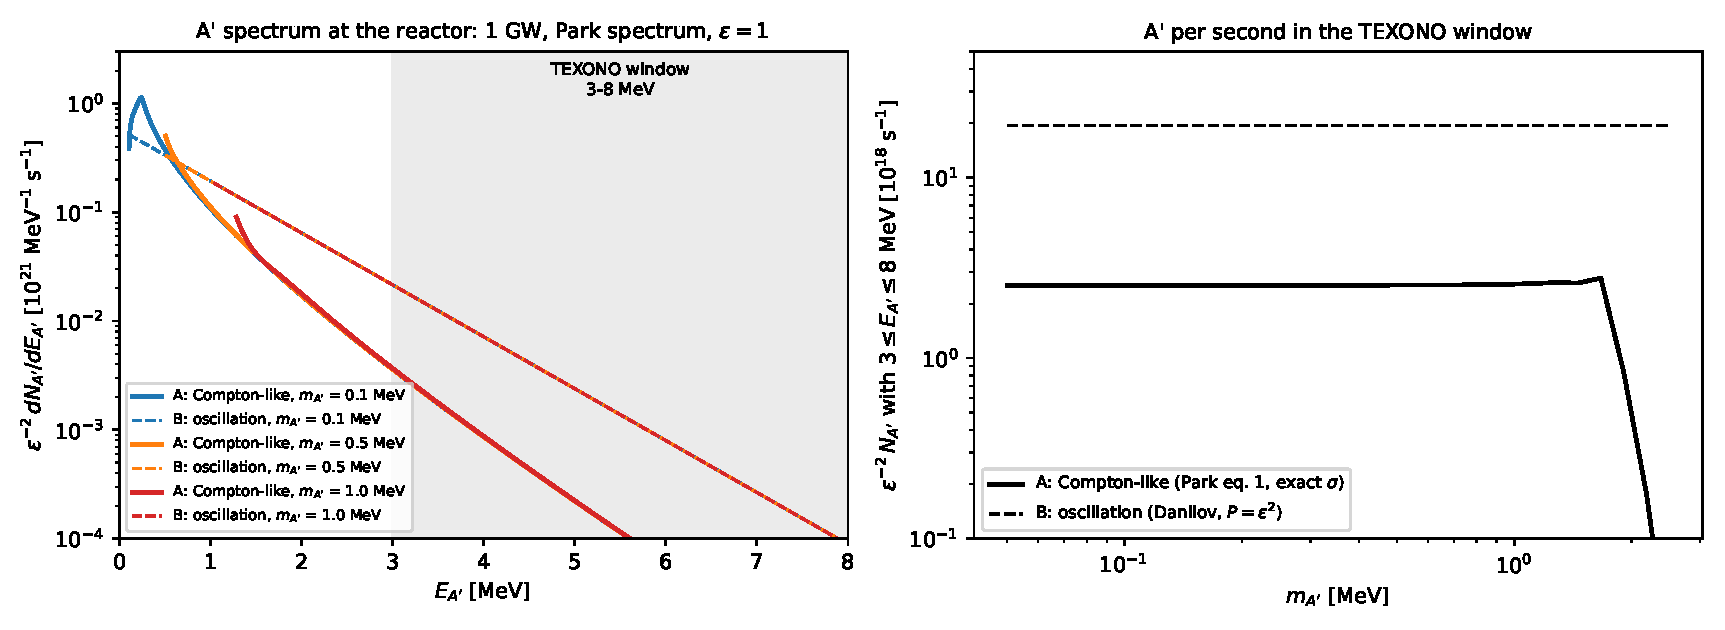
\includegraphics[width=\textwidth]{../work/fig_dN_dE_two_models.pdf}
\caption{Expected number of $\Ap$ produced per second at a 1~GW reactor with Park's spectrum, $\eps=1$. Left: spectrum
$\dd\dot N_{\Ap}/\dd E_{\Ap}$ for mechanism A (Compton-like, eq.~\eqref{eq:park1} with the exact cross section, solid)
and mechanism B (oscillation, eq.~\eqref{eq:danilov} with $P=\eps^2$ and $E_{\Ap}=E_\gamma$, dashed) for
$m_{\Ap}=0.1,0.5,1$~MeV; grey band: TEXONO's 3--8~MeV window. Right: $\Ap$ per second in that window versus mass.
B exceeds A by $7.7$ in the window; both are $\propto\eps^2$.}
\label{fig:two}
\end{figure}

\section{The detection factor $2/3$}
Park's eq.~(6) writes $\dd\sigma_{\Ap e\to\gamma e}/\dd E_r\approx\tfrac23\eps^2\,\dd\sigma_C/\dd E_r$; Lou--Wu eq.~(11)
repeats it; Danilov et al.\ call it irrelevant; the \emph{v3} report uses $P_{X\to\gamma}\sigma_\KN$ with no $2/3$.
Computed here with the same explicit matrices for the inverse process $\Ap(q)+e\to\gamma+e$, integrated over the CM angle,
$E_{\Ap}=3$~MeV, $M=0.01$~MeV:
\begin{equation}
\frac{\sigma_T}{\eps^2\sigma_\KN}=0.99999,\qquad
\frac{\sigma_L}{\eps^2\sigma_\KN}=3\times10^{-5},\qquad
\frac{\tfrac13(2\sigma_T+\sigma_L)}{\eps^2\sigma_\KN}=0.66667 .
\end{equation}
The $2/3$ is the unpolarized average: two transverse polarizations that scatter like photons and one longitudinal that
does not. It applies only to an unpolarized $\Ap$ beam. The reactor beam is not unpolarized:
oscillation/direct emission gives transverse $\Ap$ only (Danilov: longitudinal production is $\propto m_X^2/E^2$), and
Compton-like production, computed here from the explicit longitudinal vector, gives a longitudinal fraction
$\sigma_L/\sigma_{\rm tot}=0.010$ at $(E,M)=(3,0.1)$~MeV, $0.195$ at $(3,0.5)$, $0.078$ at $(3,1)$, $0.211$ at $(8,1)$
(Fig.~\ref{fig:long}). The correct detection cross section is
\begin{equation}
\sigma_{\rm det}=f_T\,\sigma_T+f_L\,\sigma_L,\qquad
\frac{\sigma_T}{\eps^2\sigma_\KN}=0.98\text{--}1.00,\quad
\frac{\sigma_L}{\eps^2\sigma_\KN}=0.02\text{--}0.31\quad (M=0.5\text{--}1,\ E_{\Ap}=3\text{--}8~{\rm MeV}),
\end{equation}
with $f_{T,L}$ the produced fractions. For $M\lesssim0.1$~MeV this is $\eps^2\sigma_\KN$ to $1\%$: factor 1, not $2/3$.
Danilov is right, Park is wrong, and Lou--Wu's eq.~(11) is a correct statement about an unpolarized beam applied to a
beam that is not. In $\eps$ the $2/3$ is a $10\%$ effect ($\eps\propto N^{-1/4}$); it matters for the bookkeeping,
not for the exclusion plot.

\begin{figure}[t]\centering
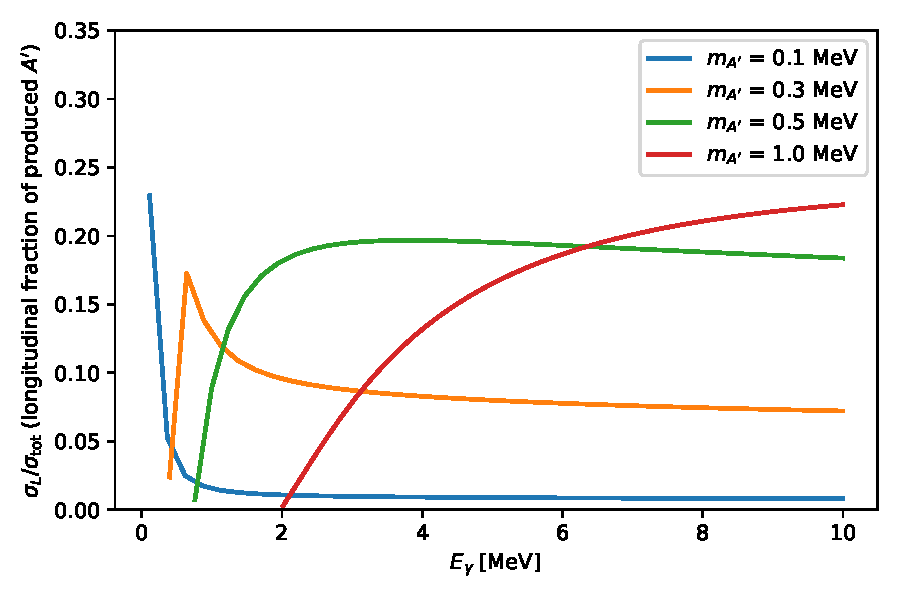
\includegraphics[width=0.62\textwidth]{../work/fig_longitudinal_fraction.pdf}
\caption{Longitudinal fraction of Compton-produced $\Ap$, from the explicit $\xi_L$ contraction integrated over
$[x_-,x_+]$. Not $\propto M^2/E_\gamma^2$: near threshold and for $M\gtrsim0.3$~MeV it is 10--25\%.}
\label{fig:long}
\end{figure}

\section{The formula to use}
For the number of $\Ap$ per unit energy arriving at a detector at distance $R$, per second, for $m_{\Ap}\gg m_\gamma$
and away from the resonance $m_{\Ap}\approx m_\gamma$:
\begin{equation}
\boxed{\;
\frac{\dd\Phi_{\Ap}}{\dd x}=\frac{1}{4\pi R^2}\left[\eps^2\,\frac{m_{\Ap}^4}{m_{\Ap}^4+x^2\Gamma_{\rm tot}^2}\,S_\gamma(x)\,f(x)
\;+\;\int\dd E\,S_\gamma(E)\,\frac{1}{\sigma_{\rm tot}(E)}\frac{\dd\sigma(E,x)}{\dd x}\right]
\;}
\label{eq:final}
\end{equation}
where the first term is eq.~\eqref{eq:danilov} (dominant; $f(x)$ is Demidov's secondary-photon factor if the second
term is not kept explicitly --- do not count both), $\dd\sigma/\dd x$ is eq.~\eqref{eq:dsdx} with eq.~\eqref{eq:F}, and
$\sigma_{\rm tot}$ is the XCOM total for the core material. The detector rate is then $N_e T\int\dd x\,(\dd\Phi/\dd x)\,
\sigma_{\rm det}(x)$ with $\sigma_{\rm det}$ as in the previous section. The \emph{v3} report implements the first term
only, with $\sigma_{\rm det}=\eps^2\sigma_\KN$; that is the right leading order. The \emph{v2} report and Park implement
the second term only; the Spanish note implements the second term with the wrong cross section.

Two normalisation choices in \texttt{apuntes/} are not errors but must be stated: the TEXONO event cap is $197.2$
(Park, $1.96\sigma$ two-sided) or $195.7$ (Danilov, one-sided $95\%$, used by \emph{v3}), and Danilov multiply it by
the anti-Compton suppression factor 6 to $1174.1$ (also used by Du et al.); \emph{v3} does not.

\section{What was checked and what was not}
\label{sec:receipt}
Checked, with assertions: the explicit-matrix $|\mathcal M|^2$ against \emph{v2}, deNiverville and Smirnov; the Ward
identity; the KN limit; the exact range and threshold; the note's eqs.~(18)--(20), (40), (50), (52) and the fold of (50) with the spectrum; the \emph{v2}
primitive $G(b)$; the KN total by quadrature; the polarization-resolved inverse cross sections; the window counts and
spectra of the two mechanisms, including that the integral of eq.~\eqref{eq:park1} over $E_{\Ap}$ returns the photon
number; Park's photon integral.

Not checked: the Gondolo--Raffelt total (paper not in the folder; \emph{v2}'s own check stands at $7\times10^{-14}$);
Park's generator and \emph{v2}'s fold code (neither available; the Figure~1 and Figure~2 values above are read by eye
from the rasters, $\pm30\%$); the XCOM/NIST attenuation numbers (recalled from
\emph{v2}); Du's and Demidov's Monte Carlos; the resonance region $m_{\Ap}\approx m_\gamma$; bound-electron and
reactor-transport effects; anything in deNiverville beyond eqs.~(18)--(20) and in NEON beyond its eq.~(2).

\medskip\noindent\sloppy
Run receipt: 21 September 2026, \texttt{work/.venv/bin/python work/check\_cross\_section.py} (numpy 2.5.2, sympy 1.12,
scipy 1.18.1, Python 3 system, venv with marimo 0.24.2); output in \texttt{work/check\_cross\_section.log}, last line
\texttt{ALL ASSERTIONS PASSED}; numbers in \texttt{work/check\_cross\_section\_out.json}; figures by
\texttt{marimo export html work/figures\_cross\_section.py}.

\begin{thebibliography}{9}\small
\bibitem{park} H.~K.~Park, Phys.\ Rev.\ Lett.\ 119, 081801 (2017). \texttt{papers\_reactor\_dark\_photon/01}.
\bibitem{danilov} M.~Danilov, S.~Demidov, D.~Gorbunov, Phys.\ Rev.\ Lett.\ 122, 041801 (2019). \texttt{02}.
\bibitem{deniv} P.~deNiverville, H.-S.~Lee, Y.-M.~Lee, arXiv:2011.03276, eqs.~(18)--(20). \texttt{03}.
\bibitem{smirnov} M.~Smirnov et al., Phys.\ Rev.\ D 104, 116024 (2021), eqs.~(3)--(4). \texttt{04}.
\bibitem{du} M.~Du, J.~Liu, X.-P.~Wang, T.~Wu, Phys.\ Rev.\ D 109, 055041 (2024). \texttt{05}.
\bibitem{neon} NEON Collaboration, Phys.\ Rev.\ Lett.\ 134, 021802 (2025), eq.~(2). \texttt{06}.
\bibitem{demidov} S.~Demidov, D.~Gorbunov, A.~Polonski, arXiv:2512.17652. \texttt{07}.
\bibitem{louwu} Y.~Lou, L.~Wu, arXiv:2606.08487, eqs.~(8), (11), App.~A. \texttt{08}.
\end{thebibliography}
\end{document}
